% Copyright 2004 by Till Tantau <tantau@users.sourceforge.net>.
%
% In principle, this file can be redistributed and/or modified under
% the terms of the GNU Public License, version 2.
%
% However, this file is supposed to be a template to be modified
% for your own needs. For this reason, if you use this file as a
% template and not specifically distribute it as part of a another
% package/program, I grant the extra permission to freely copy and
% modify this file as you see fit and even to delete this copyright
% notice. 

\documentclass{beamer}

% There are many different themes available for Beamer. A comprehensive
% list with examples is given here:
% http://deic.uab.es/~iblanes/beamer_gallery/index_by_theme.html
% You can uncomment the themes below if you would like to use a different
% one:
%\usetheme{AnnArbor}
%\usetheme{Antibes}
%\usetheme{Bergen}
%\usetheme{Berkeley}
%\usetheme{Berlin}
%\usetheme{Boadilla}
%\usetheme{boxes}
%\usetheme{CambridgeUS}
%\usetheme{Copenhagen}
%\usetheme{Darmstadt}
%\usetheme{default}
%\usetheme{Frankfurt}
%\usetheme{Goettingen}
%\usetheme{Hannover}
%\usetheme{Ilmenau}
%\usetheme{JuanLesPins}
%\usetheme{Luebeck}
\usetheme{Madrid}
%\usetheme{Malmoe}
%\usetheme{Marburg}
%\usetheme{Montpellier}
%\usetheme{PaloAlto}
%\usetheme{Pittsburgh}
%\usetheme{Rochester}
%\usetheme{Singapore}
%\usetheme{Szeged}
%\usetheme{Warsaw}

\title{Implementación de un Transmisor de ISDB-T Abierto Bajo el Paradigma de Radio Definida por Software}

% A subtitle is optional and this may be deleted
%\subtitle{Optional Subtitle}

\author{Santiago Castro \and Javier Hernandez}
% - Give the names in the same order as the appear in the paper.
% - Use the \inst{?} command only if the authors have different
%   affiliation.

\institute[Universidad de la Republica] % (optional, but mostly needed)
{
  Universidad de la Republica\\
  Facultad de Ingenieria\\
  Instituto de Ingenieria Electrica
 
}
% - Use the \inst command only if there are several affiliations.
% - Keep it simple, no one is interested in your street address.

\date{Proyecto Fin de Carrera, 2018}
% - Either use conference name or its abbreviation.
% - Not really informative to the audience, more for people (including
%   yourself) who are reading the slides online

\subject{Theoretical Computer Science}
% This is only inserted into the PDF information catalog. Can be left
% out. 

% If you have a file called "university-logo-filename.xxx", where xxx
% is a graphic format that can be processed by latex or pdflatex,
% resp., then you can add a logo as follows:

\pgfdeclareimage[height= 1.0cm]{university-logo}{logo_univ.pdf}
\logo{\pgfuseimage{university-logo}}


% Delete this, if you do not want the table of contents to pop up at
% the beginning of each subsection:
\AtBeginSubsection[]
{
  \begin{frame}<beamer>{Temario}
    \tableofcontents[currentsection,currentsubsection]
  \end{frame}
}

% Let's get started
\begin{document}

\begin{frame}
  \titlepage
\end{frame}

\begin{frame}{Temario}
  \tableofcontents
  % You might wish to add the option [pausesections]
\end{frame}

% Section and subsections will appear in the presentation overview
% and table of contents.
%\section{Introducción}
\section{Introducción}

\begin{frame}{Introducción}
\begin{block}{Conceptos básicos}
	\begin{itemize}
		\item {	La Televisión Digital en Uruguay.}
		\item {	La experiencia gr-isdbt como gran antecedente. }
		\item {	¿Que es el paradigma Radio Definida por Software (SDR)?	}
	\end{itemize}
\end{block}

\end{frame}

\section{La Norma ISDB-T}
%\subsection{Conceptos generales sobre la norma}*
\begin{frame}{La Norma ISDB-T}
	\begin{block}{Las Normas o Estándares}
	\begin{itemize}
		%\subsection{Las Normas o Estandares}
		\item {	¿Qué es una norma?}
		\item { ¿Qué alcance tiene la norma? }
		\item {	¿Cómo se define una norma?	}
	\end{itemize}
	\end{block}
	\begin{block}{La Norma ISDB-T}
	\begin{itemize}
		%\subsection{Las normas de Television Digital}
		\item {	Normas existentes en la actualidad}
		\item { Los países y las normas que usan }
		\item {	Uruguay y la definición por ISDB-T	}
	\end{itemize}
	\end{block}
\end{frame}

\begin{frame}{La Norma ISDB-T}
%\begin{block}{Conceptos básicos}
\begin{figure}
	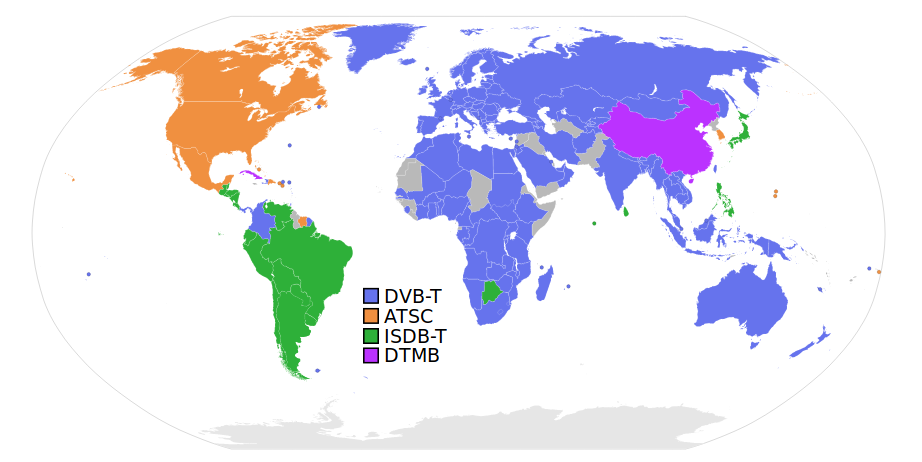
\includegraphics[scale=0.35]{Standards}
	%\caption{Distribución de las normas de TVD en el mundo}
\end{figure}
%\end{block}

\end{frame}

%\subsection{ISDB-T, la norma japonesa-brasilera de televisión}*
\begin{frame}{La Norma ISDB-T}
	\begin{block}{ISDB-T}
	\begin{itemize}	
		\item {	La entrada de datos}
		\item { Las capas jerárquicas}
		\item {	Robustecimiento a nivel datos y a nivel portadora}
		\item { OFDM }
	\end{itemize}
\end{block}
\end{frame}

%		\begin{frame}{Blocks}
%			\begin{block}{Block Title}
%			You can also highlight sections of your presentation in a block, with it's own title
%			\end{block}
%			\begin{theorem}
%			There are separate environments for theorems, examples, definitions and proofs.
%			\end{theorem}
%			\begin{example}
%			Here is an example of an example block.
%			\end{example}
%		\end{frame}

\section{Radio Definida por Software}

%\subsection{SDR, surgimiento y utilizacion actual}

\begin{frame}{Radio Definida por Software}
\begin{block}{SDR (Software Defined Radio)}
	\begin{itemize}
		%\subsection{ISDB-T (International Standard for Digital Broadcasting - Terrestrial)}	
		\item {	¿Qué es? }
		\item { ¿Qué ventajas tiene? }
		\item { La utilización de SDR en gr-isdbt-Tx}
	\end{itemize}
\end{block}
\end{frame}

%\subsection{GNU Radio}
\begin{frame}
\frametitle{Radio Definida por Software}
\begin{columns}
	\column{0.5\textwidth}
	\begin{itemize}	
		\item { Software de código abierto para SDR}
		\item {	Flowgraphs y Bloques }
		\item { La creación de bloques personalizados }
	\end{itemize}
	\column{0.5\textwidth}
	\begin{figure}
		
\includegraphics[scale=0.25]{sdr}
		%\caption{GNU Radio}
	\end{figure}
\end{columns}
\end{frame}

\begin{frame}{GNU Radio}
	\begin{figure}
	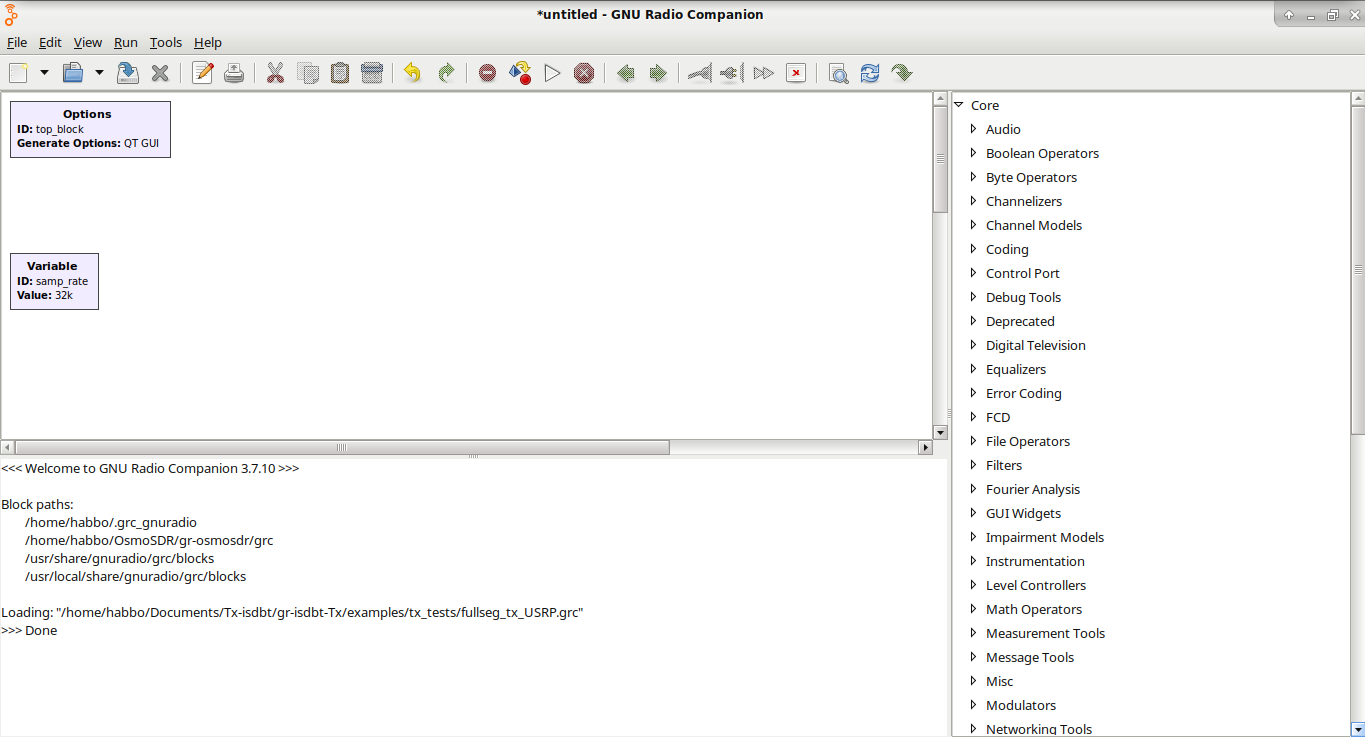
\includegraphics[scale=0.22]{grc}
	%\caption{GNU Radio framework}
	\end{figure}
\end{frame}

%\subsection{El hardware utilizado}
\begin{frame}
\frametitle{El hardware utilizado}
\begin{columns}
	\column{0.5\textwidth}
		\begin{itemize}	
			\item {Ettus Research B100}
		\end{itemize}
		\begin{figure}
		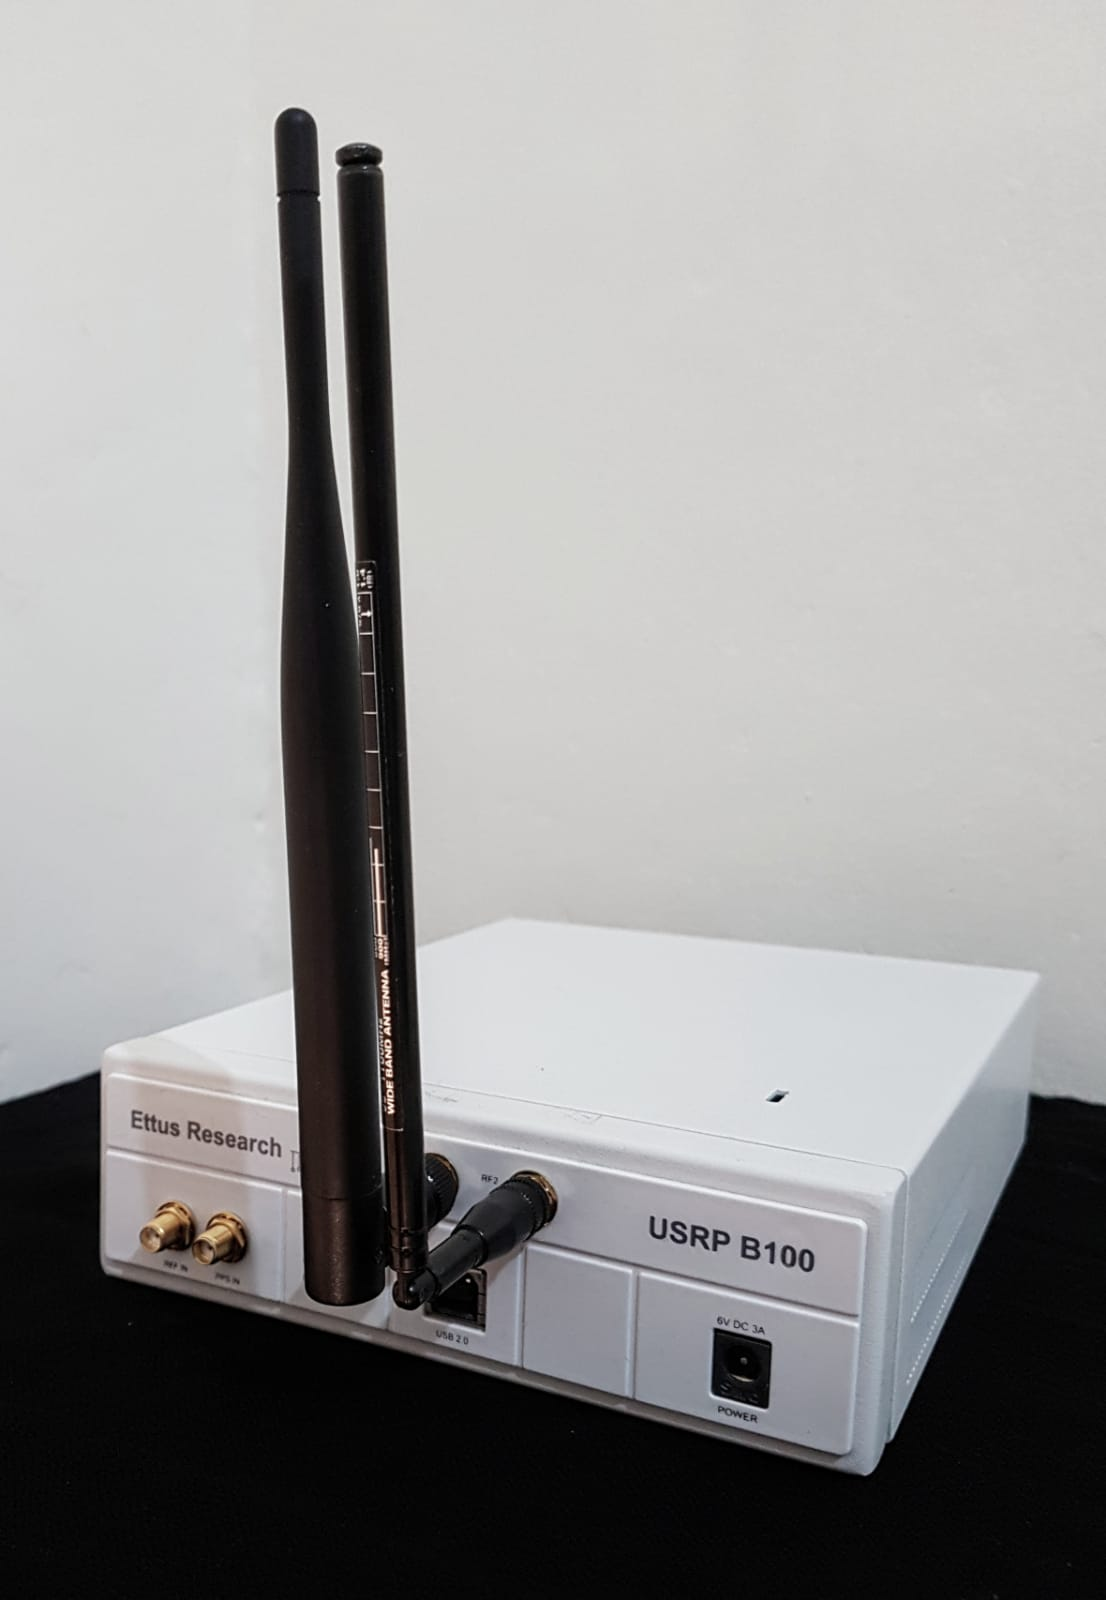
\includegraphics[scale=0.10]{usrp_foto}
		%\caption{USRP B100}
		\end{figure}
	\column{0.5\textwidth}
		\begin{itemize}	
			\item { Antenas de uso múltiple}
		\end{itemize}
		\begin{figure}
			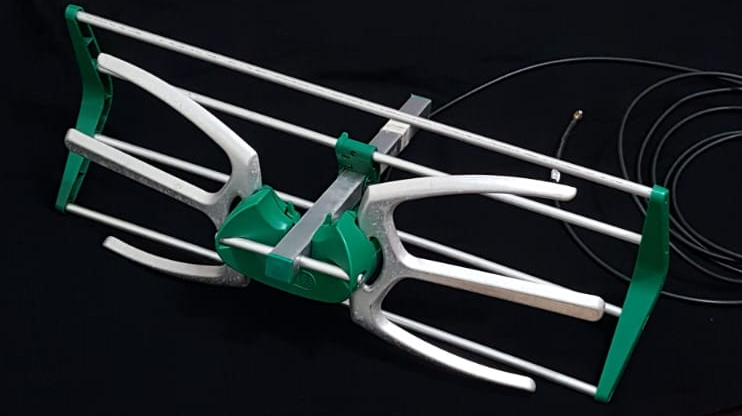
\includegraphics[scale=0.20]{antena}
			%\caption{Antena para la banda de TV}
		\end{figure}
\end{columns}
\end{frame}
\section{gr-isdbt-Tx Un transmisor ISDB-T implementado en SDR}

%\subsection{Comienza seccion 4}
\begin{frame}{gr-isdbt-tx}
\begin{figure}
	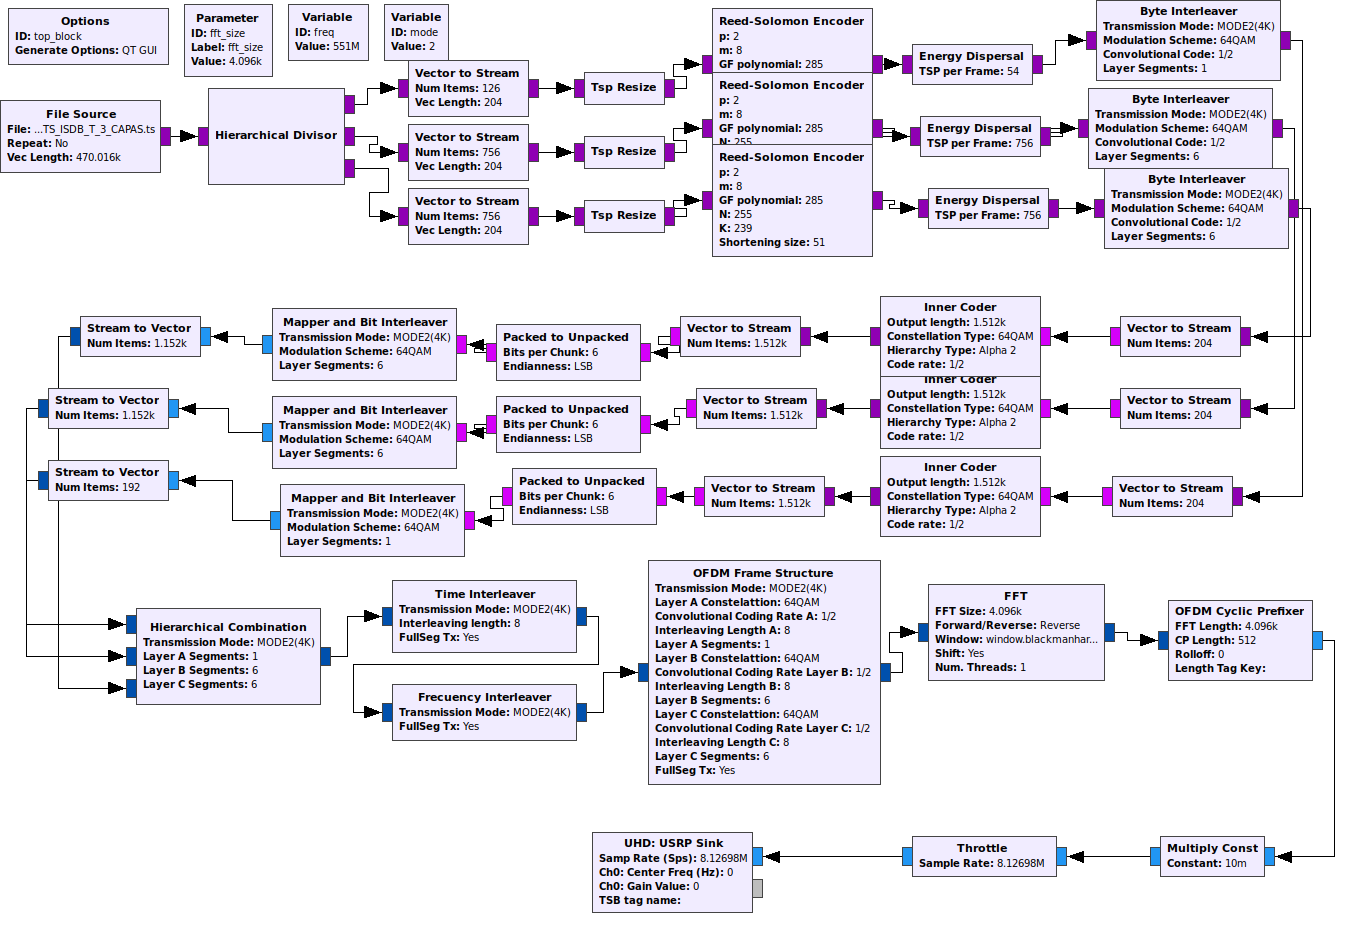
\includegraphics[scale=0.20]{flowgraphEdited}
	\caption{Esquema de bloques de gr-isdbt-Tx en GNU Radio}
\end{figure}
\end{frame}

%\subsection{La entrada de datos}
\begin{frame}
\frametitle{El divisor jerárquico}
	\begin{itemize}	
		\item { Separa TS válidos por capa}
		\item {	Descarta TSP nulos }
		\item { Cada TS continúa a procesamiento individual }
	\end{itemize}
	\begin{figure}
		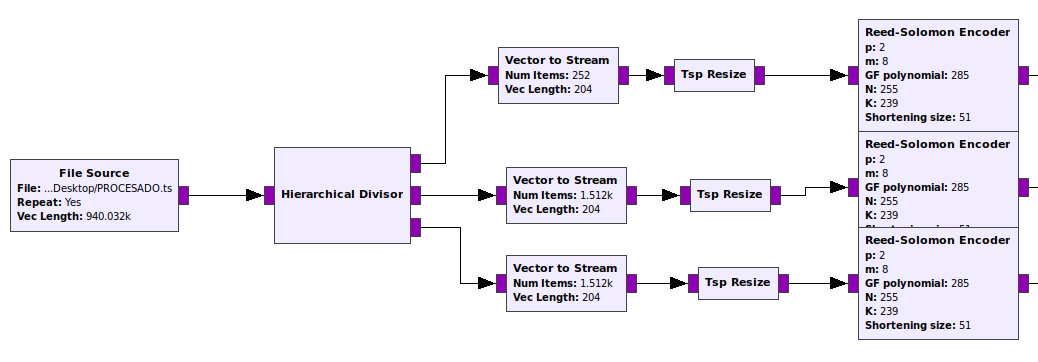
\includegraphics[scale=0.25]{h_div}
		\caption{Divisor jerárquico}
	\end{figure}
\end{frame}

%\subsection{El robustecimiento a nivel de datos}
\begin{frame}
\frametitle{El robustecimiento a nivel de datos}
\begin{itemize}	
	\item { Se aplican códigos correctores de errores a nivel de bits y bytes}
	\item {	Para aumentar la eficacia del código, se utilizan entrelazamientos}
	\item { Entrelazar implica agregar un retardo, que debe ser corregido }
\end{itemize}
\begin{figure}
	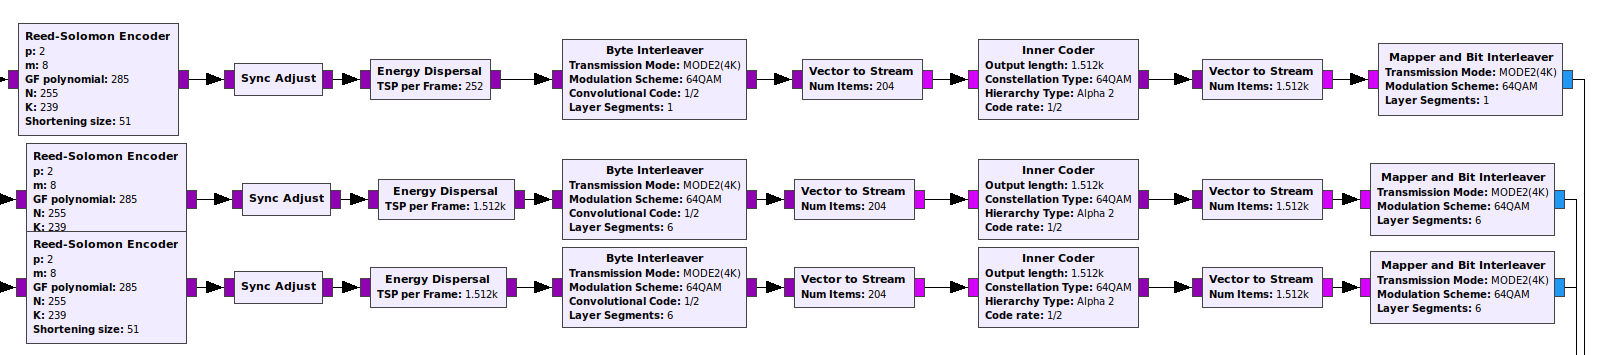
\includegraphics[scale=0.22]{rob_datos}
	\caption{Codificación de canal}
\end{figure}
\end{frame}
%\subsection{Mapeo y recombinación jerárquica}
\begin{frame}
\frametitle{Recombinacion jerárquica}
\begin{itemize}	
	\item { Se vuelven a entrelazar los datos, ahora mapeados en números complejos}
	\item {	Para aumentar la eficacia del código, se utilizan entrelazamientos}
	\item { Entrelazar implica agregar un retardo, que debe ser corregido }
\end{itemize}
\begin{figure}
	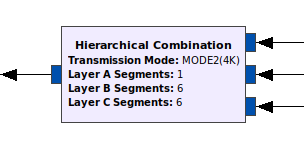
\includegraphics[scale=0.55]{h_conv}
	\caption{Combinador jerárquico}
\end{figure}
\end{frame}
%\subsection{El robustecimiento a nivel de portadoras}
\begin{frame}
\frametitle{El robustecimiento a nivel de portadoras}
\begin{itemize}	
	\item { Se realizan entrelazados en tiempo y frecuencia}
	\item {	El objetivo es mitigar los efectos del canal}
	\item { No es vital, pero mejora el desempeño en canales ruidosos }
\end{itemize}
\begin{figure}
	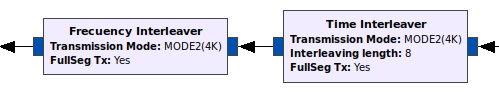
\includegraphics[scale=0.55]{rob_port}
	\caption{Bloques de entrelazamiento}
\end{figure}
\end{frame}
%\subsection{Formación del cuadro OFDM}
\begin{frame}
\frametitle{Formación del cuadro OFDM}
\begin{itemize}	
	\item { Se ubican los datos dentro de cada símbolo}
	\item {	Se agregan las portadoras piloto. Información de transmisión en las portadoras TMCC}
	\item { Agregamos portadoras dispersas para estimar el efecto del canal }
\end{itemize}
\begin{figure}
	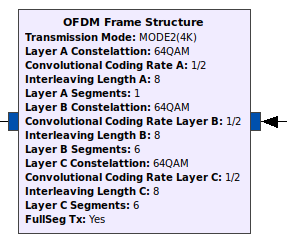
\includegraphics[scale=0.4]{bloque_ofdm}
	\caption{GNU Radio}
\end{figure}
\end{frame}

\begin{frame}
\frametitle{Formación del cuadro OFDM}
\begin{itemize}	
	\item { Ubicación de Portadoras de Datos y Portadoras Piloto}
	\item {	Agregamos información de transmision en las portadoras TMCC}
	\item { Agregamos portadoras dispersas para estimar el efecto del canal }
	\item { Agregamos portadoras auxiliares para enviar información extra (opcional) }
\end{itemize}
\begin{figure}
	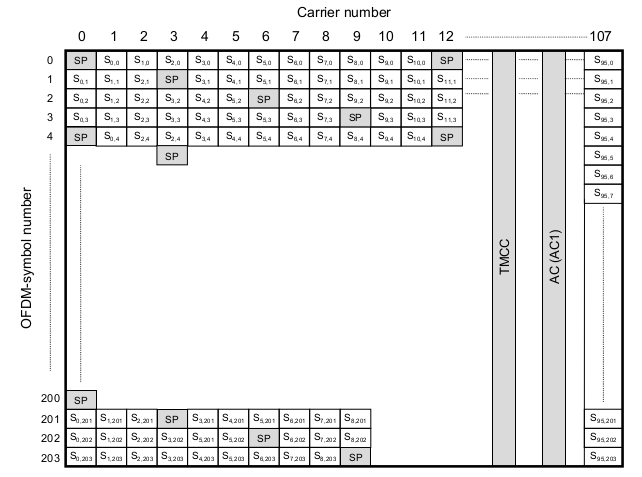
\includegraphics[scale=0.3]{ofdm_frame}
	%\caption{GNU Radio}
\end{figure}
\end{frame}
%\subsection{La puesta en el aire}
\begin{frame}
\frametitle{La puesta en el aire}
\begin{itemize}	
	\item { Mediante la transformada de Fourier pasamos al dominio del tiempo}
	\item {	Se agrega el prefijo cíclico}
	\item { Normalizamos los datos para la entrada al USRP }
	\item { Se determinan los parámetros de transmision en el equipo }
\end{itemize}
\begin{figure}
	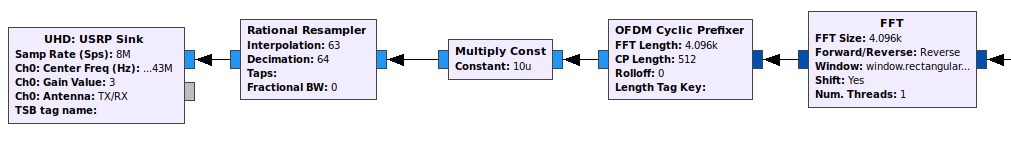
\includegraphics[scale=0.3]{final_tx}
	%\caption{GNU Radio}
\end{figure}
\end{frame}
\section{Pruebas y Resultados}

%\subsection{Pruebas en ambiente controlado}
\begin{frame}{Pruebas en ambiente controlado}
\begin{block}{Caso ideal, conexión directa}
	\begin{itemize}
		%\subsection{ISDB-T (International Standard for Digital Broadcasting - Terrestrial)}	
		\item { Se decodificaron las tres capas exitosamente }
		\item { Verificamos la funcionalidad básica del sistema }
	\end{itemize}
\end{block}

\begin{block}{Caso ruidoso, simulamos perdidas en el canal}
	\begin{itemize}
		%\subsection{ISDB-T (International Standard for Digital Broadcasting - Terrestrial)}	
		\item {	Observamos el efecto de los bloques correctores de errores }
		\item { Encontramos un umbral de ruido tolerable }
	\end{itemize}
\end{block}
\end{frame}

\begin{frame}{Pruebas en ambiente controlado}
	\begin{figure}
		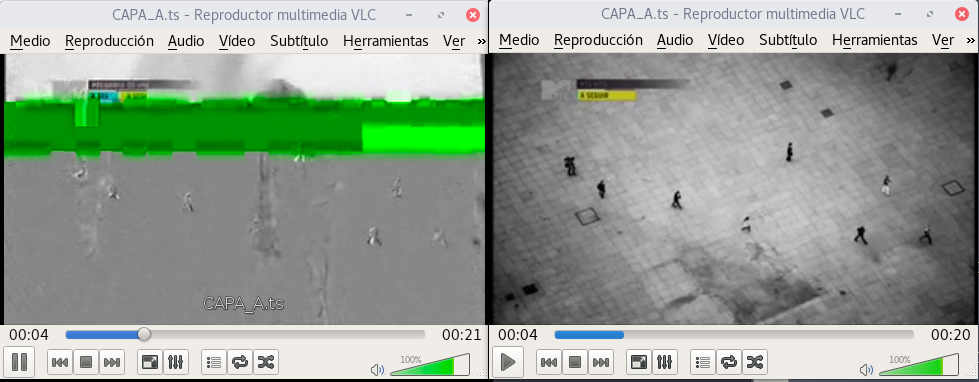
\includegraphics[scale=0.35]{calidad_imagen}
		\caption{Umbral de ruido encontrado en ambiente controlado}
	\end{figure}
\end{frame}

%\subsection{Pruebas en canal real}

\begin{frame}{Pruebas en canal real}
\begin{block}{Pruebas contra gr-isdbt en otra PC}
	\begin{itemize}	
		\item { Encontramos  }
		\item { Verificamos la funcionalidad basica del sistema }
	\end{itemize}
\end{block}

\begin{block}{Pruebas contra equipo comercial Rohde-Schwarz}
\begin{columns}
	\column{0.5\textwidth}
	\begin{itemize}	
		\item {	Observamos la constelación recibida, detectamos un bug importante }
		\item { Primeras diferencias notorias entre gr-isdbt-tx y los transmisores comerciales }
	\end{itemize}
	\column{0.5\textwidth}
	\begin{figure}
		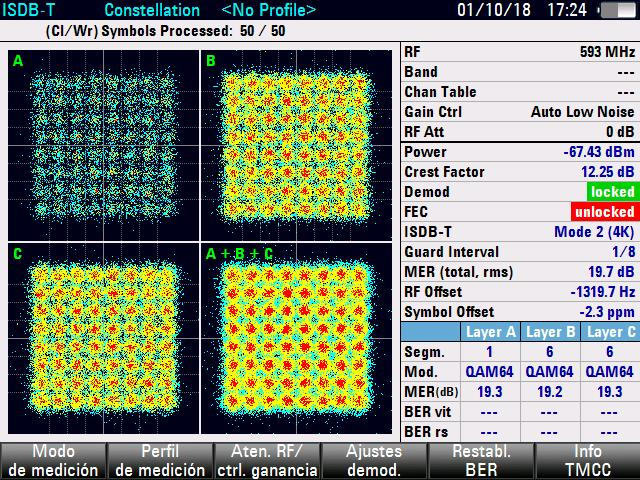
\includegraphics[scale=0.25]{constelacion_eth}
		\caption{GNU Radio}
	\end{figure}
\end{columns}
\end{block}
\end{frame}

\begin{frame}{Pruebas en canal real}
\begin{block}{Pruebas contra televisor comercial}
	\begin{itemize}	
		\item { Comprobamos que funcionan las tres capas correctamente  }
		\item { Se cumple con los objetivos planteados al principio del proyecto }
	\end{itemize}
\end{block}

	\begin{figure}
	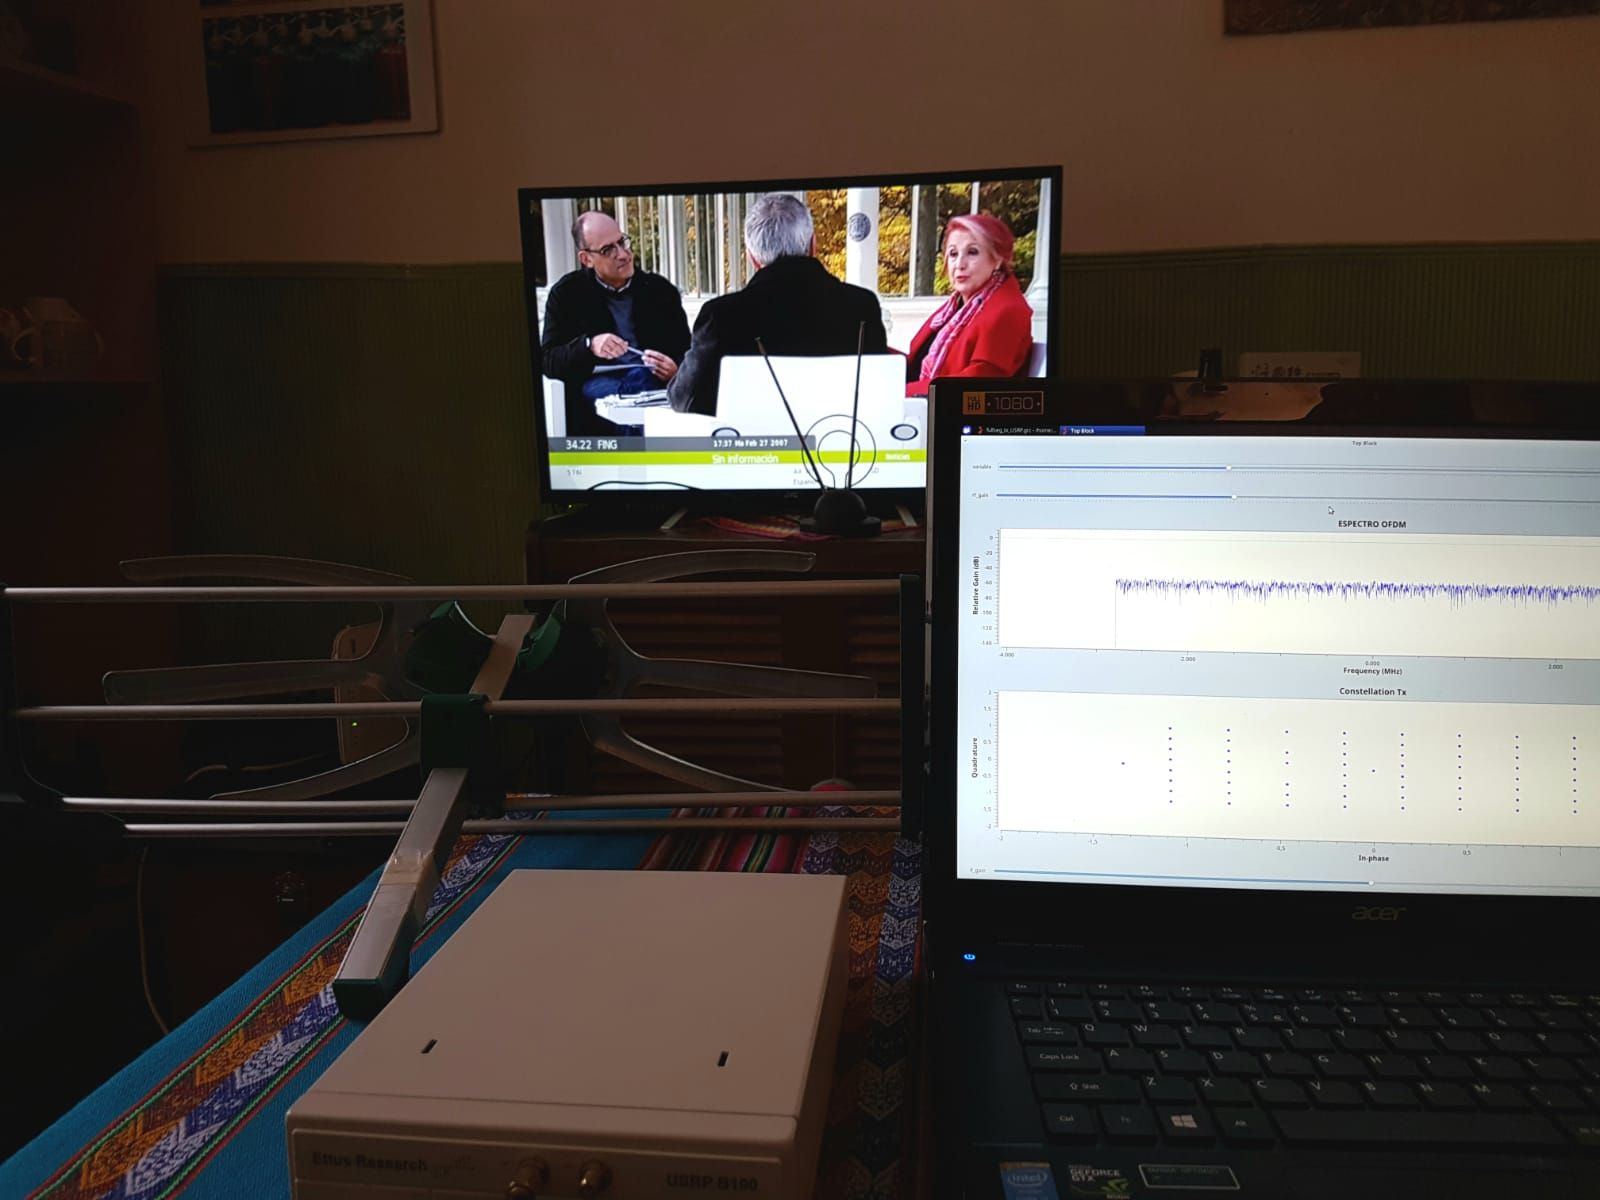
\includegraphics[scale=0.11]{contra_tele}
	\caption{GNU Radio}
	\end{figure}

\end{frame}
\section{Conclusiones y Trabajo a Futuro}

%\subsection{Conclusiones}

\begin{frame}{Conclusiones y Trabajo a Futuro}
\begin{block}{Conclusiones}
	\begin{itemize}
		\item { Se logro implementar un transmisor de TVD basado en SDR }
		\item { Se cumplió con el objetivo de transmitir de forma exitosa contra televisores comerciales }
		\item { El código quedo publicado, para que cualquiera pueda descargarlo, analizarlo y mejorarlo}
	\end{itemize}
\end{block}
\end{frame}

%\subsection{Trabajo a Futuro}

\begin{frame}{Conclusiones y Trabajo a Futuro}
\begin{block}{Trabajo a Futuro}
	\begin{itemize}
		\item { Optimizacion del código para mejorar performance }
		\item { Adaptar la entrada de datos para abarcar videos de diversos formatos }
		\item { Mejorar la documentación del codigo}
		\item { Presentación del código en conjunto con gr-isdbt para el repositorio GNU Radio}
	\end{itemize}
\end{block}
\end{frame}
%\section{Espacio Para Preguntas}*

\begin{frame}{Muchas Gracias!}
\begin{block}{Espacio Para Preguntas}

\end{block}
\end{frame}

\end{document}


